\chapter{Gramatyki}

\section{Teoria języków i gramatyk formalnych}
Przed zdefiniowaniem języka formalnego należy zdefiniować pojęcie alfabetu.
\begin{definicja}
 Przez alfabet rozumiemy dowolny skończony zbiór symboli $\mathnormal{V = \{a_{1},...,a_{n}\}}$. Skończone ciągi (nazywane słowami) z powtórzeniami elementów zbioru $\mathnormal{V}$ zapisywane są w postaci $\mathnormal{a_{1}a_{2}a_{3}a_{1}}$. Dla każdego $\mathnormal{a \in V}$ słowo jednoliterowe składające się z pojedynczego symbolu $\mathnormal{a}$ jest identyfikowane z tym symbolem i oznaczane przez $\mathnormal{a}$. Zbiór wszystkich słów nad alfabetem $\mathnormal{V}$ oznaczany jest przez $\mathnormal{V^{*}}$.
\end{definicja}
\begin{definicja}
 Niech $\mathnormal{V}$ będzie dowolnym alfabetem. Każdy podzbiór $\mathnormal{L}$ zbioru $\mathnormal{V^{*}}$ nazywamy językiem nad alfabetem $\mathnormal{V}$. Operacje wyprowadzenia można podzielić na dwie grupy. Do pierwszej z nich należą operacje teoriomnogościowe: operacje sumy, przecięcia, różnicy. Do drugiej grupy należą operacje złożenia i odbicia zwierciadlanego.\newline
\end{definicja}

\begin{definicja}
	$\textbf{Złożeniem}$ języków $L_{1}$ oraz $L_{2}$ nad alfabetem $\Sigma$ nazywamy język $X: L_{1} \cdot L_{2} = \{x \cdot y | x \in L_{1} \wedge y \in L_{2}\} $
\end{definicja}

\begin{definicja}
	W podobny sposób definiujemy potęgę języka $L$:
	\begin{itemize}
		\item $L^{\emptyset} = \{\epsilon \}$
		\item $L^{n+1} = L^{n} \cdot L$
		\item $L^{0} = \{ \emptyset \}$
	\end{itemize}
\end{definicja}

\begin{definicja}
	$\textbf{Odbiciem zwierciadlanym słowa}$ $ w = a_{1}...a_{n} \in A^{*}$ nazywamy słowo $\overline{w} = a_{n}...a_{1}$. $\newline$ Odbiciem zwierciadlanym języka $L \subset A^{*}$ nazywamy język $L = \{ \overline{w} \in A^{*} : w \in L \} $
\end{definicja}


\noindent Przez gramatykę należy rozumieć systematyczny opis wybranego języka naturalnego. Opis musi obejmować jego składnię (syntaktykę), znaczenie (semantykę) i fonologię, czyli dźwiękowy system języka. Reguły składni określają regularności rządzące kombinacjami słów, semantyka bada znaczenie słów i zdań, a fonologia wyróżnia dźwięki i ich dopuszczalne zestawienia w opisywanym języku. Teoria języków formalnych bada tylko syntaktyczne własności języków.  


\begin{definicja}
	Gramatyką nazywamy czwórkę $\mathnormal{G = \langle \sum, V, P, S \rangle}$ gdzie: 
	\begin{itemize}
	\item $\sum$ jest alfabetem,
	\item $\mathnormal{V}$ jest skończonym zbiorem zmiennych (symboli nieterminalnych) rozłączonym z $\sum$,
	\item $\mathnormal{S \in V}$ jest wyróżnionym symbolem generującym (symbol startowy),
	\item $\mathnormal{P \subseteq ( \sum \bigcup V )^{+} \times (\sum \bigcup V)^{*}}$ - jest skończonym zbiorem reguł (produkcji)
	\end{itemize}
\end{definicja}

 \begin{definicja}
	Produkcje gramatyki określają relację $\textbf{bezpośredniego wyprowadzenia}$ $\Rightarrow$ na słowach nad alfabetem $\mathnormal{( \sum \bigcup V )}$ następująco: \newline x$\Rightarrow$y wtedy i tylko wtedy, gdy istnieją słowa $x_{0}$ i $x_{1}$ oraz reguła $ \alpha \rightarrow \beta $ gramatyki $\mathnormal{G}$ takie, że $\mathnormal{x=x_{0} \alpha x_{1}}$ i $\mathnormal{y=x_{0} \beta x_{1}}$.
\end{definicja}

 \begin{definicja}
	$\textbf{Wyprowadzeniem}$ słowa $y$ ze słowa $x$ w gramatyce $G$ $(x \Rightarrow^{*y})$ nazwa się każdy ciąg słów $x_{0}, ..., x_{n}n \ge 0$, taki że $x_{i} \Rightarrow x_{i+1}$ dla $i=0, ..., n-1$ oraz $x_{0} = x $ i $x_{0} = x $ i $ x_{n} = y $. Relacja wyprowadzenia jest zwrotnym i przechodnim domknięciem  $(\Rightarrow^{*})$ relacji bezpośredniego wyprowadzenia $(\Rightarrow)$.
\end{definicja}

\begin{definicja}
	Język $L(G)$ generowany przez gramatykę $G$ definiowany jest jako zbiór wszystkich słów nad alfabetem $\Sigma$, dla których istnieje wyprowadzenie z symbolu startowego $S$, czyli: $L(G) = \{ w \in \Sigma^{*} | S \Rightarrow^{*} w \}$.
\end{definicja}

 

\subsection{Języki regularne}
Dla języka regularnego musi istnieć automat o skończonej liczbie stanów, który potrafi zdecydować czy dane słowo należy do języka.

\begin{pojecie}
	Gramatyka prawostronnie liniowa, to taka, w której wszystkie produkcje mają postać: $ A \rightarrow \alpha B$ lub $ A \rightarrow \alpha$ dla $ A, B \in V$ i $ \alpha \in \sum *$ 
\end{pojecie}

\begin{definicja}
	Niech $\Sigma$ będzie skończonym alfabetem. Rodzina $REG(\Sigma^{*})$ języków regularnych nad alfabetem $\Sigma$ to najmniejsza, w sensie inkluzji, rodzina $R$ języków taka, że:
	\begin{enumerate}
		\item $\emptyset \in R$, dla każdego $a \in \Sigma, \{a\} \in R$ - są to tak zwane języki atomowe,
		\item jeśli $X, Y \in R$ to $X\bigcup Y\in R, X \cdot Y \in R$
		\item jeśli $X \in R$, to $X^{*} = \bigcup_{n=0}{\infty} \space X^{n} \in R$
	\end{enumerate}
	Z definicji wynika, że $\{ \epsilon \} = \emptyset^{*} \in R$.
\end{definicja}
Języki regularne tworzone są z języka pustego i języków jednoelementowych złożonych z jednej litery za pomocą skończonej liczby operacji sumy, konkatenacji i gwiazdki.
Konkatenacja i suma języków skończonych to języki skończone, natomiast operacja gwiazdki na dowolnym języku różnym od $\emptyset$ i $ \{\epsilon \} $ powoduje powstanie języka nieskończonego.

\begin{przyklad}
	Przykłady języków regularnych: 
	\begin{itemize}
		\item $ \{a,b\} \cdot \{a,b\} = \{aa, ab, bc, bb\}$ jest regularny, ponieważ jest zbudowany ze złożenia dwóch języków jednoelementowych
		\item $ \{a,aa\} \cdot \{a,aa\} = \{aa, aaa, aaaa\}=\{a^{2}, a^{3}, a^{4}\}$ jest regularny, ponieważ jest złożony ze złożenia dwóch języków złożonych z konkatenacji języków skończonych
		\item $ X=\{a\}, X^{*}=\{\epsilon, a, a^{2}, a^{3}, ...\} $
		\item $ \{a \}  \Cup  \{aa\} 
		= \{a, aa\} $ jest regularny, ponieważ jest zbudowany z sumy dwóch języków złożonych z języków jednoelementowych
	\end{itemize}
\end{przyklad}

\begin{pojecie}
	Deterministycznym i skończonym automatem $A$ nazywamy piątkę $\mathnormal{\langle \sum, Q, F, \delta, q_{0} \rangle}$, w której:
	\begin{itemize}
		\item $\sum$ jest zbiorem skończonym nazywanym alfabetem
		\item $Q$ jest zbiorem skończonym nazywanym zbiorem stanów (rozłącznym z $\sum$)
		\item $F \subseteq Q$ jest podzbiorem stanów końcowych (akceptujących, terminalnych)
		\item $q_{0} \in Q$ jest wyróżnionym stanem początkowym
		\item funkcja $\delta$ zwana jest funkcją przejścia lub zmiany stanu, $\delta: Q \times \Sigma \rightarrow Q$
	\end{itemize}
Funkcję $\delta$ łatwo można rozszerzyć do funkcji $\delta^{*}: Q \times \Sigma^{*} \rightarrow Q $ w następujący sposób:
\begin{itemize}
	\item $\delta^{*}(q,\epsilon) = q$
	\item $\delta^{*}(q, Xw) = \delta^{*}(\delta(q,x), w) $
\end{itemize}
\end{pojecie}


\begin{definicja}
	Język $L \subset \sum^{*}$ jest rozpoznawalny (akceptowalny) wtedy i tylko wtedy, gdy istnieje automat skończony 
	$ A = \mathnormal{\langle \sum, Q, F, \delta, q_{0} \rangle}$ taki, że: $L = \{ w \in \Sigma^{*} : \delta^{*}(q_{0}, w) \in F \} $.
\end{definicja}


\begin{twierdzenie}
	Dla dowolnego języka $L \subset \sum^{*}$ następujące warunki są równoważne:
	\begin{itemize}
		\item Język $L$ jest regularny
		\item Istnieje gramatyka $G$ prawostronnie liniowa taka, że $L = L (G) $ - język $L$ jest generowany przez gramatykę $G$
		\item Istnieje automat skończony $\underline{A} = \mathnormal{\langle \sum, Q, F, \delta, q_{0} \rangle}$,
		 taki że $L = L (\underline{A})$ - to znaczy, że język $L$ jest akceptowany przez $\underline{A}$
	\end{itemize}
\end{twierdzenie}

Automat jest urządzeniem, który posiada nieskończoną taśmę wejściową, służącą tylko do czytania słów nad alfabetem $\sum$. Pod wpływem przeczytanej ostatnio informacji (litery słowa na wejściu) automat zmienia swój stan. Automat skończony wczytuje dane słowo znaku po znaku i zgodnie z funkcją przejścia podejmuje decyzję o zmianie swojego stanu. Po wczytaniu całego słowa sprawdza, czy znajduje się w jednym ze stanów akceptujących. Jeżeli automat znajdzie się w stanie akceptującym to powiem, że automat akceptuje słowo. W przeciwnym wypadku mówimy, że słowo nie jest zaakceptowane przez automat. Schemat automatu może zostać zaprezentowany jako graf skierowany, którego wierzchołkami są stany, a krawędzie są etykietowane literami alfabetu wyjściowego. 

\begin{center}
	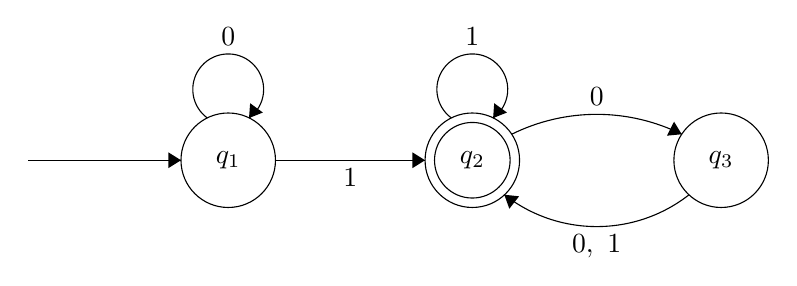
\begin{tikzpicture}[scale=0.2]
	\tikzstyle{every node}+=[inner sep=0pt]
	\draw [black] (16.3,-29.1) circle (3);
	\draw (16.3,-29.1) node {$q_{1}$};
	\draw [black] (31.8,-29.1) circle (3);
	\draw (31.8,-29.1) node {$q_{2}$};
	\draw [black] (31.8,-29.1) circle (2.4);
	\draw [black] (47.6,-29.1) circle (3);
	\draw (47.6,-29.1) node {$q_{3}$};
	\draw [black] (30.477,-26.42) arc (234:-54:2.25);
	\draw (31.8,-21.85) node [above] {$1$};
	\fill [black] (33.12,-26.42) -- (34,-26.07) -- (33.19,-25.48);
	\draw [black] (3.6,-29.1) -- (13.3,-29.1);
	\fill [black] (13.3,-29.1) -- (12.5,-28.6) -- (12.5,-29.6);
	\draw [black] (45.567,-31.289) arc (-51.92551:-128.07449:9.513);
	\fill [black] (33.83,-31.29) -- (34.15,-32.18) -- (34.77,-31.39);
	\draw (39.7,-33.81) node [below] {$0,\mbox{ }1$};
	\draw [black] (14.977,-26.42) arc (234:-54:2.25);
	\draw (16.3,-21.85) node [above] {$0$};
	\fill [black] (17.62,-26.42) -- (18.5,-26.07) -- (17.69,-25.48);
	\draw [black] (19.3,-29.1) -- (28.8,-29.1);
	\fill [black] (28.8,-29.1) -- (28,-28.6) -- (28,-29.6);
	\draw (24.05,-29.6) node [below] {$1$};
	\draw [black] (34.297,-27.451) arc (116.3725:63.6275:12.163);
	\fill [black] (45.1,-27.45) -- (44.61,-26.65) -- (44.16,-27.54);
	\draw (39.7,-25.69) node [above] {$0$};
	\end{tikzpicture}
\end{center}

Powyższy automat akceptuje język $ L = \{ w \in \{0,1\}^{*} | w $ zawiera przynajmniej jedną jedynkę i parzystą liczbę zer na końcu $ \} $.

\subsection{Języki bezkontekstowe - gramatyki bezkontekstowe}

W języku naturalnym jakim jest język polski gramatyka ustala zasady poprawnego budowania zdań. Dzięki temu rozmawiające ze sobą osoby są w stanie się zrozumieć. Języki bezkontekstowe są rodziną szerszą niż omówione wcześniej języki regularne. Język bezkontekstowy to taki język formalny, dla którego istnieje niedeterministyczny automat ze stosem, który potrafi zdecydować czy dany łańcuch należy do języka. Równoważnie dla takiego łańcucha musi istnieć gramatyka bezkontekstowa. Gramatyki bezkontekstowe generują napisy poprzez sekwencję przepisywać, która ma strukturę drzewa. Ze względu na strukturę drzewiastą gramatyki bezkontekstowe nadają się bardzo dobrze do opisu syntaktyki języków programowania.

\begin{definicja}
Gramatyka jest bezkontekstowa, gdy wszystkie jej produkcje są postaci $\mathnormal{A \rightarrow \beta}$, gdzie $\mathnormal{A \in V, \beta \in (\sum \bigcup V)^{*}}$
\end{definicja}

\begin{przyklad}
	Gramatyka $G = (\{a,b  \}, {S}, {S \rightarrow aSb | \epsilon }, S) $ generuje język $ \{a^{n}b^{n}\}$ Język wygenerowany przez gramatykę nie jest regularny.
\end{przyklad}

Tak jak wyrażenia regularne mają równoważny z nimi automat - automat skończony, tak gramatyki bezkontekstowe mają swój odpowiednik maszynowy, jest to automat ze stosem. Automat ze stosem to automat skończony, który został wyposażony w dodatkową pamięć w postaci stosu - jest to lista działająca na zasadzie first in, last out. Nowa symbole mogą być dopisywana lub czytane jedynie na wierzchołku listy. Automaty skończone dysponują skończoną pamięcią, niezależną od długości danych wejściowych. W przypadku automatów ze stosem, dysponujemy także nieskończoną pamięcią, dzięki czemu można rozpoznawać szerszą klasę języków. Tą klasą są języki bezkontekstowe.

\begin{definicja}
	Automatem ze stosem nazywamy system $A_{s} = \langle \sum, Q, F, \Gamma, \delta, q_{0}, Z_{0} \rangle $, gdzie:
	\begin{itemize}
		\item $\sum$ - skończony zbiór symboli wejściowych (alfabet)
		\item $Q$ - skończony zbiór stanów
		\item $\Gamma$ - skończony zbiór symboli na stosie (alfabet stosowy)
		\item $q_{0} \in Q$ - wyróżniony stan początkowy
		\item $Z_{0} \in \Gamma$ - symbol początkowy na stosie - wyróżniony symbol stosowy
		\item $F \subseteq Q$ - jest podzbiorem stanów końcowych
		\item $\delta$ - funkcja przejścia
	\end{itemize}
\end{definicja} 

Maszyna będąc w określonym stanie czyta literę słowa wejściowego oraz sprawdza, jaki symbol znajduje się na wierzchołku stosu. Na tej podstawie podejmowana jest decyzja o zmianie stanu, następnie zdejmowany jest element z wierzchołka stosu. Na zdjętym elemencie umieszczane jest słowo złożone z symboli stosowych. 
\begin{twierdzenie}
	Dla dowolnego języka $L \subset \sum^{*}$ następujące warunki są równoważne:
	\begin{itemize}
		\item Język $L$ jest bezkontekstowy
	 	\item Istnieje gramatyka $G$ prawostronnie liniowa taka, że $L = L(G)$ - język $L$ jest generowany przez gramatykę bezkontekstową $G$
		\item Istnieje automat ze stosem $\underline{A_{s}}  = \langle \sum, Q, F, \Gamma, \delta, q_{0}, Z_{0} \rangle$,
		taki że $L = L(\underline{A})$ - to znaczy, że język $L$ jest akceptowany przez $\underline{A}$
	\end{itemize}
\end{twierdzenie}

	\begin{twierdzenie}
		Język $ L \subset \sum^{*} $ jest generowany przez gramatykę bezkontekstową wtedy i tylko wtedy gdy $L$ jest akceptowalny przez automat ze stosem.
	\end{twierdzenie}	
	
	Niech będzie dany automat ze stosem $A= \langle \sum, Q, F, \Gamma, \delta, q_{1}, Z_{0} \rangle$, który rozpoznaje język $L=\{a^{n}b^{n} | n \ge 1 \}$	
	\begin{center}
		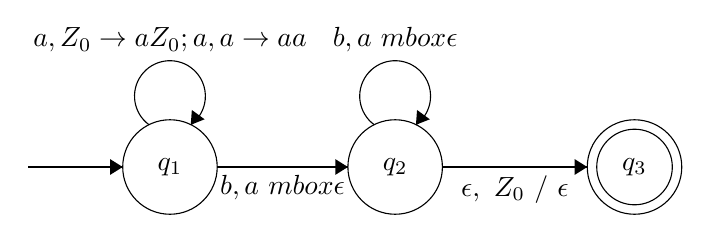
\begin{tikzpicture}[scale=0.2]
		\tikzstyle{every node}+=[inner sep=0pt]
		\draw [black] (21.6,-26.5) circle (3);
		\draw (21.6,-26.5) node {$q_1$};
		\draw [black] (51.1,-26.5) circle (3);
		\draw (51.1,-26.5) node {$q_3$};
		\draw [black] (51.1,-26.5) circle (2.4);
		\draw [black] (35.9,-26.5) circle (3);
		\draw (35.9,-26.5) node {$q_2$};
		\draw [black] (12.6,-26.5) -- (18.6,-26.5);
		\fill [black] (18.6,-26.5) -- (17.8,-26) -- (17.8,-27);
		\draw [black] (20.277,-23.82) arc (234:-54:2.25);
		\draw (21.6,-19.25) node [above] {$a, Z_0 \rightarrow aZ_0; a,a \rightarrow aa$};
		\fill [black] (22.92,-23.82) -- (23.8,-23.47) -- (22.99,-22.88);
		\draw [black] (24.6,-26.5) -- (32.9,-26.5);
		\fill [black] (32.9,-26.5) -- (32.1,-26) -- (32.1,-27);
		\draw (28.75,-27) node [below] {$b,a\mbox{ }\\mbox{ }\epsilon$};
		\draw [black] (38.9,-26.5) -- (48.1,-26.5);
		\fill [black] (48.1,-26.5) -- (47.3,-26) -- (47.3,-27);
		\draw (43.5,-27) node [below] {$\epsilon,\mbox{ }Z_0\mbox{ }/\mbox{ }\epsilon$};
		\draw [black] (34.577,-23.82) arc (234:-54:2.25);
		\draw (35.9,-19.25) node [above] {$b,a\mbox{ }\\mbox{ }\epsilon$};
		\fill [black] (37.22,-23.82) -- (38.1,-23.47) -- (37.29,-22.88);
		\end{tikzpicture}
	\end{center}

	Zapis $a,b \rightarrow c$ oznacza, że maszyna czytając ze słowa wejściowego literę $a$, może zastąpić literę $b$ na wierzchołku ciągiem symboli $c$.




\subsection{Hierarchia Chomsky'ego}
Amerykański językoznawca Noam Chomsky zaproponował cztery typy gramatyk, które maja swoją hierarchę. Hierarchia Choomsky'ego to hierarchia czterech klas języków. Są to języki: regularne, bezkontekstowe, kontekstowe i częściowo obliczalne. Każdej z tych klas przypada jeden rodzaj gramatyki. Odpowiadają im gramatyki: liniowe, bezkontekstowe, kontekstowe i rekurencyjnie przeliczalne. Tym samym klasom odpowiadają cztery różne modele obliczeniowe: automaty skończone, automaty ze stosem, maszyny Turinga (ograniczone liniowo i dowolne). 

\begin{definicja}
	Niech $\mathnormal{G = \langle \sum, V, P, S \rangle}$ będzie dowolną gramatyką.\newline
	\begin{enumerate}
		\item $\mathnormal{G}$ jest typu 1 lub jest gramatyką kontekstową wtedy i tylko wtedy, gdy wszystkie produkcje $\alpha \rightarrow \beta$ spełniają warunek $\mathnormal{|\alpha| \leqslant |\beta|}$
		\item $\mathnormal{G}$ jest typu 2 lub jest gramatyką bezkontekstową wtedy i tylko wtedy, gdy wszystkie produkcje są postaci $\mathnormal{A \rightarrow \beta}$, gdzie $\mathnormal{A \in V, \beta \in (\sum \bigcup V)^{*}}$
		\item $\mathnormal{G}$  jest typu 3 lub jest gramatyką regularną wtedy i tylko wtedy gdy jest prawostronnie lub lewostronnie liniowa.
	\end{enumerate}
\end{definicja}
Poniższy diagram przedstawia graficzną reprezentacje języków formalnych.

\begin{figure}[H]
	\centering
	\includegraphics[width=0.7\linewidth]{hierarchia}
	\caption{Hierarchia języków formalnych}
	\label{fig:hierarchia}
\end{figure}

\begin{definicja}
	Język należy do danej klasy wtedy i tylko wtedy, gdy jest możliwe zbudowanie gramatyki formalnej, która generuje dany język, a której reguły przestrzegają ograniczeń dla danej klasy.
\end{definicja}
 

\section{Gramatyki i muzyka}
Wykorzystanie gramatyki do generowania muzyki charakteryzuje się kilkoma tendencjami. Pierwszą z nich jest określenie jakim rodzajem muzyki ma dana gramatyka się zajmować. Na podstawie rodzaju muzyki należy dokonać charakteryzacji według rodzajów akordów, tempa, linii melodycznej itp. Przykładowo dla muzyki jazzowej można stworzyć produkcje, które będą tworzyły harmoniczne pasujące do siebie akordy bazujące na teorii jazzu i następstwie akordów. 

\subsection{Przykład wykorzystania gramatyk w muzyce}

Jako przykład zostanie przygotowana gramatyka, której celem będzie wygenerowanie prostej melodii bazującej na tonacji C-dur. Na gamę C-dur składają się następujące dźwięki: C, D, E, F, G, A, H. 

\begin{figure}[H]
	\centering
	\includegraphics[width=0.7\linewidth]{c_dur}
	\caption[]{Gama C-dur}
 
	\label{fig:cdur}
\end{figure}

Zapis tonacji C-dur podobnie jak A-moll (A, H, C, D, E, F, G) nie posiada znaków chromatycznych. Tonacje są pokrewne ze sobą. 

Melodia nie powinna przekraczać dwóch oktaw (dwie oktawy: C, D, E, F, G, A, H, C, D, E, F, G, A, H). Metrum melodii czyli czynnik porządkujący ugrupowania rytmicznie za pomocą regularnie powtarzających się akcentów metrycznych wyniesie 4/4 (cztery czwarte). Górna liczba metrum oznacza ile ma być w takcie jednostek miarowych oznaczonych przez liczbę dolną. Przykładowo określenie 2/4 wskazuje, że w jednym takcie mają być dwie ćwierćnuty lub wartości dające w sumie dwie ćwierćnuty. Dolna liczba wskazuje, jaka wartość nutowa jest podstawą miary taktowej. Jednostką miarową może być cała nuta, półnuta, ósemka, szesnastka i trzydziestodwójka. Aby utworzyć melodię kolejność nut musi być ułożona w taki sposób aby utwór był przyjemny dla ucha. Jeżeli nuty zostaną użyte w sposób losowy melodia nie będzie brzmiała dobrze.

\begin{przyklad}
	Rozważmy gramatykę $\mathnormal{G = \langle \sum, V, P, S \rangle}$ gdzie:
	\begin{itemize}
		\item $ \sum = \{ n.k; n \in \langle 0, 87 \rangle, k \in \langle 1, 3 \rangle \} $ - wyrażenie $n.k$ będzie rozpatrywane jako nuta gdzie $n$ oznaczać będzie wysokość nuty, a $k$ długość trwania  dźwięku 1 - cała nuta , 2 - półnuta, 3 - ćwierć nuta. 
		\item $V = \{ S, Beg, Mid, End\}$
		\item Zbiór produkcji $P$ jest następujący: 
		
		$\mathnormal{S \rightarrow Beg\ Mid\ End\ }$\\
		$\mathnormal{Beg \rightarrow 47'1\ 49'1\ 51'1\ 52'1\ }$\\
		$\mathnormal{Beg \rightarrow 52'2\ 56'2\ 59'2\ 57'2\ }$\\
		$\mathnormal{Beg \rightarrow Beg\ 52'2\ 54'2\ 56'2\ 54'2\ Mid\ }$\\
		$\mathnormal{Beg \rightarrow 47'1\ 49'1\ 51'1\ 52'1\ 54'3\ End\ }$\\
		$\mathnormal{Mid \rightarrow Beg\ 52'2\ 56'2\ End\ }$\\
		$\mathnormal{Mid \rightarrow 54'2\ 56'1\ 54'1\ 52'2\ 47'2\ }$\\
		$\mathnormal{Mid \rightarrow Mid\ 47'2\ 52'2\ 56'1\ 57'1\ 56'1\ 52'1\ Beg\ }$\\
		$\mathnormal{Mid \rightarrow 56'2\ 52'1\ 54'1\ 56'2\ }$\\
		$\mathnormal{End \rightarrow Mid\ Beg\ 54'2\ 51'2\ 52'3\  }$\\
		$\mathnormal{End \rightarrow 52'2\ 52'2\ 51'2\ 52'3\ }$\\
		$\mathnormal{End \rightarrow Beg\ 52'2\ 54'2\ 52'3\ End\ }$\\
		$\mathnormal{End \rightarrow 52'4\ }$\\
		$\mathnormal{End \rightarrow 42'2\ 40'3\ }$\\
		$\mathnormal{End \rightarrow 49'1\ 47'1\ 49'1\ 51'1\ 52'3\ End\ }$\\
	\end{itemize}
\end{przyklad}

Za pomocą języka Python można zautomatyzować proces wyprowadzeń. W tym celu będzie pomocna biblioteka nltk, która służy  do pracy z przetwarzaniem języka naturalnego. 

	\begin{lstlisting}[caption={Generowanie wyprowadzeń z gramatyki bezkontekstowej},captionpos=b]
	from nltk import CFG
	from nltk.parse.generate import generate
	import re
	from music21 import *
	notes = ['C', 'C#', 'D', 'D#', 'E', 'F', 'F#', 'G', 'G#', 'A', 'A#', 'B']
	num_notes = 127
	num_octaves = 10
	octave_count = 0
	num_to_note = dict()
	
	for i in range(0, num_notes+1):
	# print "{} {} {}".format(i, octave_count, notes[i%len(notes)])
	num_to_note.update({str(i): notes[i % len(notes)]+str(octave_count)})
	if i % 12 == 11:
	octave_count += 1
	
	gramma = """
	S -> Beg Mid End 
	Beg -> '47.1 49.1 51.1 52.1'
	Beg -> '52.2 56.2 59.2 57.2'
	Beg -> Beg '52.2 54.2 56.2 54.2' Mid
	Beg -> '47.1 49.1 51.1 52.1 54.3' End
	Mid -> Beg '52.2 56.2' End
	Mid -> '54.2 56.1 54.1 52.2 47.2'
	Mid -> Mid '47.2 52.2 56.1 57.1 56.1 52.1' Beg 
	Mid -> '56.2 52.1 54.1 56.2'
	End -> Mid Beg '54.2 51.2 52.3' 
	End -> 52'2 52'2 51'2 52'3
	End -> Beg '52.2 54.2 52.3' End
	End -> '52.4'
	End -> '42.2 40.3'
	End -> '49.1 47.1 49.1 51.1 52.3' End
	"""
	environment.set("musescoreDirectPNGPath",     "/usr/bin/musescore")
	environment.set("musicxmlPath",     "/usr/bin/musescore")
	environment.set("midiPath",     "/usr/bin/lilypond")
	
	conv = converter.subConverters.ConverterLilypond()
	
	grammar = CFG.fromstring(gramma)
	track_array = []
	for track in generate(grammar, n=5, depth=3):
	track_array.append(' '.join(track))
	print (track)
	
	tracks_notes = []
	
	for tr in track_array:
		s1 = stream.Stream()
		for n in re.findall(r'\S+', tr):
		s1.append(note.Note(num_to_note.get(str(n.split('.')[0])), quarterLength=int(n.split('.')[1])))
		tracks_notes.append(s1)
 
	
	
	for i, k in enumerate(tracks_notes):
		print(k)
		conv.write(k, fmt='lilypond', fp='/mnt/c/Users/Lukasz/MGR_Code/Grammar/examples/' + str(i), subformats=['png', 'midi'])	
	\end{lstlisting}	
	Do powyższego przykładu został stworzony interfejs graficzny. Za pomocą interfejsu można wygenerować przykładowe melodie.
	\begin{figure}[H]
		\centering
		\includegraphics[width=0.5\linewidth]{grammar_parser_gui}
		\caption{Interfejs aplikacji}
		\label{fig:grammarparsergui}
	\end{figure}
	
	Interfejs pozwala na wprowadzenie ilości wyprowadzeń oraz głębokości, która jest istotna przy procesie wyprowadzania słów. Zbyt duża głębokość prowadzi do zapętlenia. Po ustaleniu odpowiednich liczb należy wcisnąć przycisk "Generuj".
	
	\begin{figure}[H]
		\centering
		\includegraphics[width=0.7\linewidth]{grammar_parser_gui_results}
		\caption{Wyniki dla głębokości równej 4 oraz liczbie iteracji równej 3}
		\label{fig:grammarparserguiresults}
	\end{figure}

	Po pomyślnym wyprowadzeniu słów program wyświetla wyniki w nowym oknie. 
	



\subsection{Programy wykorzystujące gramatyki}

$\textbf{MusicMachine.io}$ - system stworzony przez Johna Leszczynskiego. Jest to przewodnik, którego celem jest akceptowanie sekwencji nut, które będą spełniały zasady stylu Cantus Firmus. Zasady, które muszą być spełnione to:

\begin{itemize}
	\item sekwencja musi się składać z co najmniej 8 nut
	\item w sekwencji musi wystąpić punk kulminacyjny - jedna nuta musi być wyższa niż pozostałe
	\item koniec sekwencji musi skończyć się na tonice (nuta zaczynająca)
	\item akceptowane interwały to: sekundy wielkie, sekundy małe, tercje, seksty oraz kwarty czyste, kwinty i oktawy
\end{itemize}

Autor oparł swój system na bibliotece napisanej w JavaScript counterpoint (John Jeszczynski jest również autorem tej biblioteki). Interfejs aplikacji jest dostępny pod adresem http://musicmachine.io.


\begin{figure}[H]
	\centering
	\includegraphics[width=0.7\linewidth]{music_machine_gui}
	\caption{Interfejs aplikacji musicmachine}
	\label{fig:musicmachinegui}
\end{figure}

Interfejs musicmachine podaje listę możliwych nut po każdym kroku. Jeżeli sekwencja wybranych nut jest zgodna z zasadami Cantus Firmus to jest akceptowana przez gramatykę umieszczoną w bibliotece. Biblioteka counterpoint wykorzystuje bibliotekę GrammarGraph. Biblioteka GrammarGraph pozwala na stworzenie gramatyki bezkonetkstowej, a następnie pozwala na wyprowadzanie słów z wcześniej zadanej gramatyki oraz potrafi zdecydować czy jakieś wyprowadzenie rzeczywiście pochodzi z gramatyki, która została zadana.

\begin{przyklad}
	Przykład gramatyki zbudowanej w oparciu o temat z Sonaty Księżycowej:
	\begin{lstlisting}[caption={}, captionpos=b]
	var jupiterGrammar = {
	     InfinitePhrase: [ 'JupiterTheme InfinitePhrase',
	         'SecondMotive InfinitePhrase' ],
	     JupiterTheme: [ '2  3  -2' ],
	     SecondMotive: [ '4  StepDown' ],
	     StepDown: [ '-2',
	         '-2  StepDown']
	}
	\end{lstlisting}
	W powyższej gramatyce można wyróżnić symbole terminalne na które składają się: 2, 3, -2, 4. Symbole terminalne oznaczają odległość między nutami - interwały. W skład symboli nie-terminalnych wchodzą: InfinitePhrase, JupiterTheme, SecondMotive, StepDown. Definicje rekurencyjne w gramatyce sprawiają, że długość wyprowadzanego słowa może być nieskończona. 
	
\end{przyklad} 

Gramatyka użyta w aplikacji musicmachine.io wygląda następująco:

\begin{lstlisting}
var upOnly = {

	// designed to be an infinite phrase
	UpPhrase: ['UpLeap DownStepPhrase UpPhrase',
	'UpStepPhrase DownPhrase'],
	
	// all choices must be prepared for a potential down leap in downphrase
	UpStepPhrase: ['Up2Phrase',
	'Up3Phrase',
	'UpLeapForwardPhrase'],
	
	// after 2, can reverse direction or continue up 2 or 3
	Up2Phrase: ['2',
	'2 Up2Phrase',
	'2 Up3Phrase'],
	
	// after 3, can reverse direction or continue up 2
	Up3Phrase: ['3',
	'3 Up2Phrase'],
	
	// up leap must be recovered with down step
	// prepare for a potential downard leap by adding another UpPhrase
	UpLeapForwardPhrase: ['2 UpLeapForward DownStepPhrase UpPhrase'],
	
	// allowed up leaps after already moving a second up
	UpLeapForward: ['4', '5'],
	
	// allowed leaps at the beginning or after a direciton change
	UpLeap: ['4', '5', '6', '8']
}
\end{lstlisting}

Symbole terminalne: 2, 3, 4, 5, 6, 8, oznaczają odległości od nut - interwały. Symbole nie-terminalne: UpPhrase, UpStepPhrase, Up2Phrase, Up3Phrase, UpLeapForwardPhrase, UpLearForward, UpLeap, DownStepPhrase, DownPhrase. Reguły obowiązują w dwóch kierunkach, dolnym i górnym. Gramatyka została zdefiniowana tylko w jednym kierunku, ponieważ kierunek przeciwny można uzyskać zamieniając symbol terminalny na przeciwny. Po każdym wyborze nuty sprawdzane jest czy sekwencja jest prawidłowa z wszystkimi zasadami Cantus Firmus. Za sprawdzanie odpowiedzialna jest poniższa funkcja:

\begin{lstlisting}
	this.isValid = function () {
		var cf = this.cf()
	
		// is it long enough
		if (cf.length < MIN_CF_LENGTH || cf.length > MAX_CF_LENGTH) {
			return false
		}
	
		// is last note tonic?
		if (Pitch(cf[cf.length - 1]).pitchClass() !== guide.tonic()) {
			return false
		} else if (Pitch(cf[0]).pitchClass() === guide.tonic()) {
		// if first note is tonic, last note should end in the same octave
		// if first note is not tonic, this is probably a first species counterpoint
			if (cf[0] !== cf[cf.length - 1]) {
				return false
			}
		}
	
		// is the penultimate note scale degree 2 or possible 7?
		if (intervalSize(cf[cf.length - 2], cf[cf.length - 1]) !== 2) {
			return false
		}
		
		// is there a unique climax (highest note is not repeated)?
		var sorted = sortPitches(cf)
		if (sorted[sorted.length - 1] === sorted[sorted.length - 2]) {
			return false
		}
		
		return true
	}
\end{lstlisting}

Poniżej pokazane zostały dwa przykłady sekwencji, w których jeden jest sekwencją, która spełnia zasady Cantus Firmus, a drugi nie. Prawidłowa sekwencja jest podświetlona na zielono.

\begin{figure}[H]
	\centering
	\includegraphics[width=0.7\linewidth]{music_machine_correct}
	\caption{Prawidłowa sekwencja CantusFirmus}
	\label{fig:musicmachinecorrect}
\end{figure}

\begin{figure}[H]
	\centering
	\includegraphics[width=0.7\linewidth]{music_machine_error}
	\caption{Nieprawidłowa sekwencja}
	\label{fig:musicmachineerror}
\end{figure}

Przykład wyprowadzenia melodii, która jest zgodna z zasadami stylu Cantus Firmus bezpośrednio z wykorzystaniem biblioteki:

\begin{lstlisting}[caption={}, captionpos=b]
var CantusFirmus = require('counterpoint').CantusFirmus
var cantus = new CantusFirmus('G major')
cantus.choices()    => ['G']
cantus.addNote('G4')

cantus.choices()    => [ 'A4', 'B4', 'C5', 'D5', 'E5', 'G5',
'F#4', 'E4', 'G3', 'B3', 'C4', 'D4' ]

cantus.addNote('E5')
cantus.choices()    => [ 'D5', 'C5' ]   

cantus.addNote('D5')
cantus.choices()    => [ 'E5', 'F#5', 'G5', 'A5', 'B5',
'C5', 'B4', 'G4', 'A4' ]
cantus.addNote('F#5')
cantus.choices()    => [ 'G5', 'E5', 'F#4', 'A4', 'B4' ]

cantus.addNote('G5')
cantus.choices()    => [ 'A5', 'B5', 'F#5', 'E5', 'G4', 'B4', 'C5', 'D5' ]

cantus.addNote('B4')
cantus.choices()     => [ 'C5', 'D5' ]
cantus.addNote('C5')
cantus.addNote('A4')

cantus.choices()     => [ 'B4', 'D5', 'E5', 'F#5', 'A5', 'G4' ]
cantus.addNote('G4')

console.log(cantus.print())

G5                  o
F#5             o
E5      o
D5          o
C5                          o
B4                      o
A4                              o
G4  o                               o
	   G4  E5  D5  F#5 G5  B4  C5  A4  G4

\end{lstlisting}

$\textbf{Kulitta}$ - framework napisany w Haskellu przez Donya Quick przeznaczony do automatycznego i algorytmicznego komponowania muzyki. System używa generatywnych gramatyk do tworzenia abstrakcyjnej struktury muzycznej, która jest następnie stopniowo ulepszana za pomocą matematycznych modeli harmonii. Kolejno specyficzne dla stylu algorytmy zamieniają harmonie w konkretny rodzaj muzyki np. chorał, jazz czy bossa nova.

\begin{figure}[H]
	\centering
	\includegraphics[width=0.7\linewidth]{kulitta_diagram}
	\caption{Struktura framerowka Kulitta}
	\label{fig:kulittadiagram}
\end{figure}
 
Kulitta korzysta ze specjalnego rodzaju gramatyk jakim są Probabilistic Temporal Graph Grammars (PTGG). PTGG są podobne do gramatyk bezkontekstowych, umożliwiają równoczesne generowanie harmonicznej i metrycznej struktury za pomocą sparametryzowanego alfabetu.  

\begin{figure}
	\centering
	\includegraphics[width=0.7\linewidth]{ptgg}
	\caption{Przykład PTGG nad symbolami funkcji akordowych, tonika (T),
		dominanta (D) i subdominanta(S), sparametryzowana przez czas trwania jako indeks górny.
		Przedstawione prawdopodobieństwa produkcyjne pochodzą z głównej części potrzebnej do generowania chorałów}
	\label{fig:ptgg}
\end{figure}